\documentclass[conference]{IEEEtran}

\usepackage{amsmath,amssymb,amsfonts}
\usepackage{algorithmic}
\usepackage{graphicx}
\usepackage{textcomp}
\usepackage{xcolor}
\usepackage{placeins}
\usepackage{hyperref}
\usepackage{gensymb}
\usepackage{subfig}
\usepackage[style=ieee]{biblatex}
\addbibresource{optimal_sailboat.bib}

\def\todo #1 {\textbf{\textcolor{red}{TODO: #1}}}

\begin{document}

\title{Optimal Control of an Autonomous Sailboat}

\author{
\IEEEauthorblockN{Tae Rugh}
\IEEEauthorblockA{\textit{Mechanical Engineering} \\
\textit{Carnegie Mellon University} \\
\href{mailto:trugh@cmu.edu}{trugh@cmu.edu}}
\and
\IEEEauthorblockN{Ben Spin}
\IEEEauthorblockA{\textit{Mechanical Engineering} \\
\textit{Carnegie Mellon University} \\
\href{mailto:bspin@cmu.edu}{bspin@cmu.edu}}
\and
\IEEEauthorblockN{Denis Alpay}
\IEEEauthorblockA{\textit{Mechanical Engineering} \\
\textit{Carnegie Mellon University} \\
\href{mailto:dkalpay@andrew.cmu.edu}{dkalpay@andrew.cmu.edu}}
\and
\IEEEauthorblockN{Samaksh Judson}
\IEEEauthorblockA{\textit{Mechanical Engineering} \\
\textit{Carnegie Mellon University} \\
\href{mailto:bspin@cmu.edu}{sjudson@andrew.cmu.edu}}
\and
\IEEEauthorblockN{Christopher Suzuki}
\IEEEauthorblockA{\textit{Mechanical Engineering} \\
\textit{Carnegie Mellon University} \\
\href{mailto:csuzuki2@andrew.cmu.edu}{csuzuki2@andrew.cmu.edu}}
}

\maketitle

\begin{abstract}
Autonomous sailboats offer a carbon-neutral solution for the shipping industry. From a control perspective, autonomous sailboats pose a unique and interesting problem because the dynamics are highly coupled to the environment such that the control is in a sense under-actuated. In this project, we leverage real-world weather predictions to develop an optimal control system for autonomous sailboats, featuring: a global route planner based on a "polar" model; a trajectory optimizer based on a 4-DoF dynamics model; and a tracking controller. Code and visualizations are available at: \href{https://github.com/taerugh/OptimalSailboat}{github.com/taerugh/OptimalSailboat}.
\end{abstract}

\begin{IEEEkeywords}
optimal control, planning, modeling, sailboat
\end{IEEEkeywords}

\section{Introduction}

\subsection{Motivation}
Given the enduring utility of winds and currents, which date back to ancient Mesopotamian transportation \cite{Carter2012Watercraft}, incorporating optimal control and route planning for sailboats presents a logical evolution in seeking carbon-neutral shipping methods. As environmental regulations tighten and fuel costs continue to rise, the shipping industry faces increasing pressure to innovate. Wind-powered solutions not only align with global sustainability goals but also offer a cost-effective alternative to fossil fuels. This is reflected by the International Maritime Organization (IMO) strategy, which aims at achieving net-zero green house gas emissions from international shipping by 2050. This includes a commitment to the promotion of alternative zero and near-zero fuels by 2030 \cite{UNCTAD2023}. By harnessing wind energy, the industry can significantly reduce dependence on oil, lowering operational costs and minimizing environmental impact. Our project aims to contribute to these efforts by developing navigational and control strategies that optimize the use of the free wind energy in the environment, thereby making green shipping a viable and competitive option in the global market.

\subsection{Background}
It has already been shown that sails could significantly cut energy use and the carbon footprint of maritime shipping \cite{Michael2014PropulsivePower}. Notably, the successful deployment of wind-powered technology in vessels like the Pyxis Ocean in 2023 underscores the practical and commercial potential of airfoil sails on large shipping vessels \cite{Lewis2023WindPowered}.

Current research largely targets yacht-like vessels \cite{ModelingCourseControl, RollController, Saoud2015OptimalSail}, reflecting the specialized interest driving this field. Our work aims to broaden the knowledge base on sailboat dynamics and utilize readily available weather data \cite{ERA5} to design optimal control and trajectory planning for autonomous vessels capable of sustained voyages. This effort aligns with our commitment to fostering a sustainable maritime shipping industry, guided by a paradigm emphasizing green energy and efficiency.

\subsection{System Overview}
We propose a controller consisting of 3 levels: A global route optimizer, which uses RRT* to find an optimal route from a starting point to an ending point with given weather conditions; a trajectory optimizer which uses direct collocation to find an optimal trajectory along the route; and a tracking controller which uses MPC to track the trajectory.

\begin{figure}[ht]
    \centering
    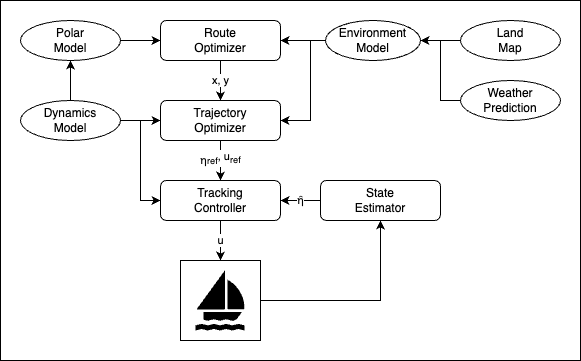
\includegraphics[width=.9\columnwidth]{fig/system_diagram.png}
    \caption{System diagram.}
    \label{fig:system_diagram}
\end{figure}

The environment is modeled with a land-ocean map and real-world weather data, described in Section \ref{section:environment}. For the route optimizer, the boat is modeled with a polar diagram, described in Section \ref{section:polar_model}, which estimates potential boat speed for given a trade wind (angle and speed). The route planner, described in Section \ref{section:route_planning}, uses the environment and polar models to generate an optimal route, consisting of a path of coordinates that the boat should follow.

The trajectory optimizer, described in Section \ref{section:trajectory_optimization}, takes this route, along with the environment information, and locally optimizes a trajectory along the route for a finite time horizon into the future. The optimized trajectory consists of reference states and control inputs.

Finally, the tracking controller, described in Section \ref{section:tracking_control}, is used to close the loop and track the reference trajectory. Both the tracking controller and trajectory optimizer use a 4 degree-of-freedom dynamics model of the sailboat described in Section \ref{section:dynamics_model}.

\section{System Modeling}

\subsection{Environment}
\label{section:environment}

\subsubsection{Weather}
We use weather data from the ERA5 reanalysis \cite{ERA5}, provided by the Climate Data Store (CDS) API from the European Centre for Medium-Range Weather Forecasts (ECMWF). From this, we can get historical weather data as well as forecasts to use for planning and as a ground truth. This source provides many data variables which may be incorporated into our model in the future, but currently we only use the wind velocity component variables. We capture the data at 0.25\degree{} latitude/longitude precision at 12 hour intervals. Then, we can linearly interpolate between these data points to get wind information at any given coordinate at any given time.

\subsubsection{Land Map}
We also use a base map from Natural Earth \cite{NaturalEarth} to identify whether a coordinate is on land or ocean. The route planner and trajectory optimizer use this data to avoid obstacles. The base map is available at varying levels of precision, which affects algorithm speed.

\begin{figure}[ht]
    \centering
    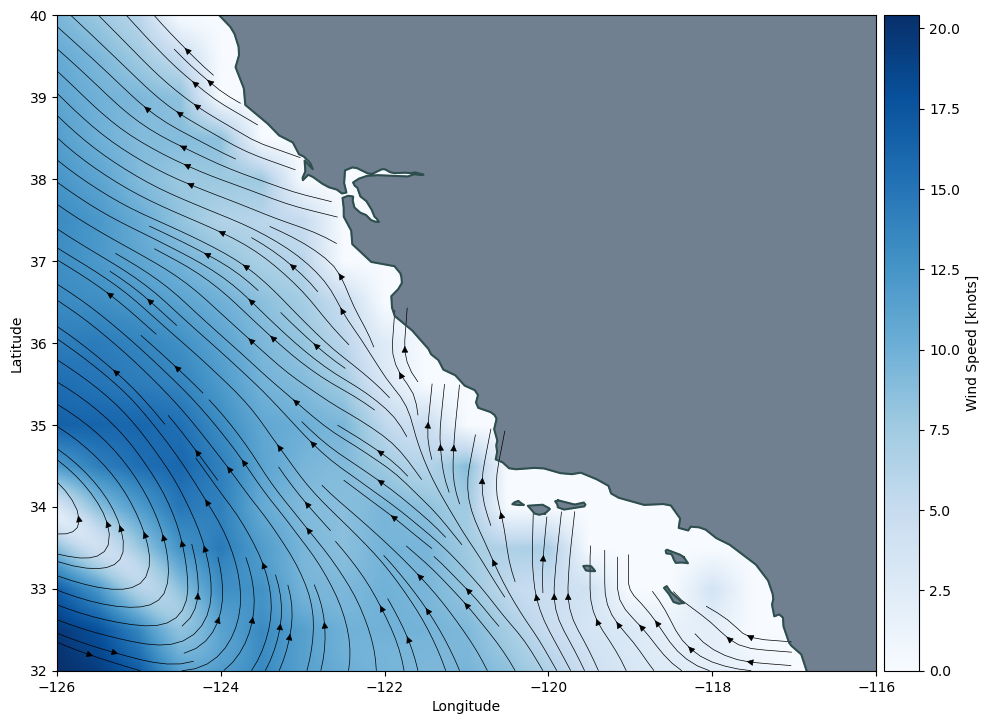
\includegraphics[width=.9\columnwidth]{fig/environment.png}
    \caption{California coast on Jan 1, 2024.}
    \label{fig:environment}
\end{figure}

\subsection{Dynamics Model}
\label{section:dynamics_model}

Our dynamics modeling closely aligns with the work of Wille et al. \cite{ModelingCourseControl}, with key modifications tailored to the specific requirements of our vessel. Notably, our approach assumes a "barge-like" hull with constant and symmetric dimensions, significantly simplifying and linearizing the modeling of damping forces. These simplifications are particularly justified considering that shipping barges typically feature large, flat bases.

We have included the visualization and definition of positive force directions from Willie et al. \cite{ModelingCourseControl} in Figure \ref{Force Directionality}

\begin{figure}[ht]
    \centering
    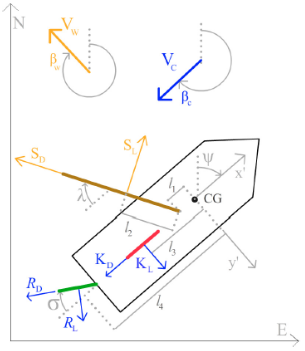
\includegraphics[width=.9\columnwidth]{fig/force_visualization_top.png}
    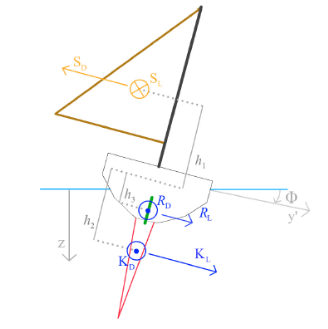
\includegraphics[width=.9\columnwidth]{fig/force_visualization_back.png}
    \caption{Directionality of forces, visualized. Figures borrowed from the work by Willie et al. \cite{ModelingCourseControl}}
    \label{Force Directionality}
\end{figure}

In addition to a "barge-like" hull, like Willie et al. \cite{ModelingCourseControl} , we borrow the assumptions of Xiao and Jouffrey \cite{Xiao2014Modeling}:

\begin{enumerate}
    \item The model assumes rigidity, disregarding any heave and pitch dynamics.
    \item The impact of waves on the ships movement is not included in the model.
    \item It is presumed that the added mass coefficients remain consistent throughout.
    \item The forces exerted by the sail, keel, rudder, and hull are calculated separately, without considering any interplay among them.
    \item The sail, keel, and rudder are treated as stiff airfoils. To simplify, the forces they generate are considered to converge at the aerodynamic center of effort.
\end{enumerate}

The sailboat is represented using a 4 DoF dynamics model. The states of the system are shown below:

\begin{align}
    \eta &= \begin{bmatrix} x & y & \phi & \psi \end{bmatrix}^\top \\
    \nu &= \begin{bmatrix} u & v & p & r \end{bmatrix}^\top
\end{align}

$\eta$ includes the position of the boat $(x,y)$, as well as roll $phi$ and yaw $psi$, all in global coordinates. $\nu$ includes the velocity of the boat $(u,v)$, the angular yaw velocity $p$, and the angular roll velocity $r$, all in the boat's body coordinates. Pitch and z displacement are ignored in this model. This 4 DoF model is a common simplification in sailboats and is justified by the fact that for most sailboats with a single hull, motion primarily occurs in the horizontal plane. Additionally, in most sailing scenarios, the dominant forces of interest are related to the boat's position (surge and sway) and orientation (yaw).

The vectoral representation of our system is as follows:

\begin{align}
   F &= M_{RB}\dot{\nu} + C_{RB}(\nu)\nu + M_A\dot{\nu_r} + C_A(\nu_r)\nu_r + D(\nu_r) \\
   &\quad + g(\eta) \notag \\
   F &= S(\eta,\nu,\lambda,V_w) + K(\eta,\nu,V_c) + R(\eta,\nu,V_c,\sigma)
\end{align}

The dynamics follow simply:

\begin{align} 
    \dot{\eta} &= J(\phi, \psi) \nu \\
    \dot{\nu} &= (M_{RB} + M_A)^{-1} \bigg(S + K + R - C_{RB}(\nu)\nu \\
                &\quad - C_A(\nu_r)\nu_r - (D_L(\nu_r) + D_Q) - g(\eta)\bigg) \notag
\end{align}

Where $S$, $R$, and $K$ represent the forces due to the sail, rudder, and keel, respectively. $D_L$ denotes the linear damping component, and $D_Q$ represents the nonlinear damping components. $M_{RB}$ and $C_{RB}$ are the real mass and Coriolis matrices, respectively, while $M_A$ and $C_A$ are the added mass and Coriolis matrices. These additions are essential to account for the additional inertial effects experienced by a body moving in water. These effects are referred to as "added" or "apparent" mass.

Linear damping $D_L$ is given by experimentally determined constants \cite{fossen2011handbook}.
\begin{align}
D_l &= \begin{bmatrix}
d_{11} & 0 & 0 & 0 \\
0 & d_{22} & 0 & 0 \\
0 & 0 & 0 & 0 \\
0 & 0 & 0 & d_{66}
\end{bmatrix}
\end{align}

The original equations for nonlinear damping in all directions are based on strip theory and are as follows:

\begin{align}
D_{qx}(\nu_r) &= \frac{1}{2} \rho_w S_{H} (1 + k) C_{F}(R_n) |u_r| u_r \\
C_{F}(R_n) &= \frac{0.075}{(\log_{10}(R_n) - 2)^2} \\
D_{qy}(v_r) &= \frac{1}{2} \rho_w \int_L C_D(x') T(x')|v_r + x' r|(v_r + x' r)  dx' \\
D_{qn}(v_r) &= \frac{1}{2} \rho_w \int_L C_D(x') T(x')x'|v_r + x' r|(v_r + x' r)  dx' \\
D_{qk}(\nu_r) &= B_{F0} \left( L_{WL} + 4.1 \frac{u_r}{\omega_{roll} L_{WL}} \right) p_r + B_{Lp} p_r u_r
\end{align}


To linearize $D_q$ however, we need to apply some key simplifications and assumptions

\begin{itemize}
\item Assume a barge-like boat with a constant Reynolds number, constant wetted surface area $S_H$, and constant lift and drag coefficients.
\item A constant characteristic \( x' = \frac{L}{2} \) assuming symmetry about the center of gravity.
\item Simplified damping forces using flat plate approximations.
\item  Draft $T$ is assumed to be constant across the hull (This aligns with our barge-like assumption).
\end{itemize}

After applying these assumptions, $ C_D$ and $T$ are found to be constant over $ x' $ . We can then integrate over the length of the hull $L$, and apply \(\tanh\) as a smooth approximation to the sign function for managing force directionality. This use of \(\tanh\) helps in capturing the continuous transition of damping forces between negative and positive velocities, thus avoiding the discontinuities typical of a step function like \(\text{sgn}\). This method assumes that the total force points in a direction determined by the characteristic \( x \) using \(\tanh\), effectively smoothing out the force direction over the characteristic \( x \). The derived equations for nonlinear damping forces based on these principles are:

\begin{align}
D_x &= \frac{1}{2} \rho_w S_H (1+k) C_F u_r^2 \cdot \tau_1 \\
D_y &= \frac{1}{2} \rho_w T C_D \left(v_r^2 L + v_r r L^2 + \frac{r^2 L^3}{3}\right) \cdot \tau_2 \\
D_n &= \frac{1}{2} \rho_w T C_D \left(\frac{v_r^2 L^2}{2} + \frac{2 v_r r L^3}{3} + \frac{r^2 L^4}{4}\right) \cdot \tau_2 \\
D_{\phi} &= B_{FO} \left(L_{WL} + 4.1 \frac{u_{bc}}{\omega_{roll} L_{WL}}\right) p_r + B_{Lp} u_{bc} p_r
\end{align}
where $\tau_1$ = \text{\(\tanh(10 u_{r})\)} and  $\tau_2$ = \text{\(\tanh(10 (v_{r} + x' r))\)}. Restoration force $g(\eta)$ are defined as:

\begin{align}
g(\eta) &= \begin{bmatrix}
0\\
0\\
\rho_w g \nabla G M_t sin(\phi)cos(\phi)\\
0
\end{bmatrix}
\end{align}

Restoration forces create a righting moment and are largely responsible for keeping the vessel upright and balanced in the water. $\nabla$ is the total displacement of the ship, $g$ is gravity, and $GM_t$ is the transverse metacentric height as outlined in \cite{ModelingCourseControl}, and defined by \cite{fossen2011handbook}.

We are modeling our sail, rudder, and keel as airfoils using NACA airfoil tools \cite{NACA} with correction terms.  NACA provides lift and drag coefficients for only between -20\degree{} and 20\degree{} angles of attack, but for our dynamics model, we need to define the full range in a differentiable form. To do this, we fit a polynomial to the NACA data, and combine this with a spline for the rest of the domain. With the spline, we are able to generate a curve that is smooth and approaches the desired value at the limits (-180\degree{} and 180\degree{}).

\begin{figure}[ht]
    \centering
    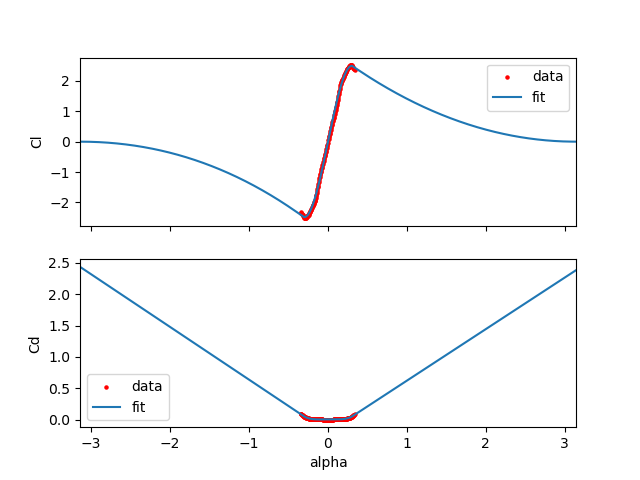
\includegraphics[width=.9\columnwidth]{fig/naca0015.png}
    \caption{Extended NACA0015 lift and drag coefficients.}
    \label{fig:naca0015}
\end{figure}

With these coefficient functions, sail, keel, and rudder forces are all modeled as:

\begin{align}
    F_L &= \frac{1}{2} \rho A C_L(\alpha)V^2 \\
    F_D &= \frac{1}{2} \rho A C_D(\alpha)V^2
\end{align}

where $\alpha$ is the angle of attack, $\rho$ is the density of air for the sail or water for the keel and rudder, $A$ is the area of the foil, $V$ is the speed relative to the foil, $C_L$ and $C_D$ are the lift and drag coefficients respectively.

\subsection{Polar Model}
\label{section:polar_model}
A polar diagram is commonly used in sailing to visualize a boat's potential speed over a range of wind speeds and relative angles. Notably, it does not reason about the controls or dynamics, and does not give any information with regards to the state or control inputs that may be used to achieve that speed. Typically, the data to make this plot is gathered by measurements in the real world, although it is possible to derive a boat polar from a dynamics model.

\begin{figure}[ht]
    \centering
    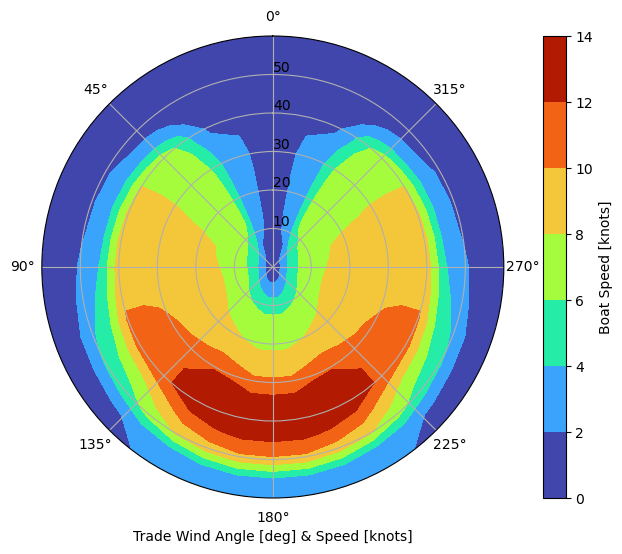
\includegraphics[width=.9\columnwidth]{fig/polar.png}
    \caption{Polar diagram for Sun Fast 40.}
    \label{fig:polar}
\end{figure}

Figure \ref{fig:polar} depicts the boat speed over trade wind angle---where 0\degree{} is directly upwind and 180\degree{} is directly downwind---and trade wind speed. Typically, wind speeds stay below 30 knots. In this region, the highest boat speeds are achieved when the wind is nearly perpendicular to the boat, at 90\degree{} and 270\degree{}. At a trade wind angle of 0\degree{}, the boat can obviously make no progress, so it must "tack" back and forth (zig-zag path) to go upwind. Additionally, even when going downwind, it is often ideal to "jibe" (again, zig-zag).

With the boat polar, we can calculate the boat speed that can be reached in a given direction subject to the environment wind conditions. By integrating this along a path, we can estimate the time it would take the sailboat to follow that path.

\section{Route Planning}
\label{section:route_planning}
Global route optimization is done using the classic sampling-based planning algorithm, Rapidly-exploring Random Trees* (RRT*) \cite{RRT-star}. RRT* relies on 2 heuristic functions, distance and cost, to find an optimal and collision-free path from a given start node to a goal node.

The distance function is used to find nearby nodes (neighbors). Since we are working in geographic coordinates, we use the Haversine formula to calculate the great-circle distance between two nodes.

The cost function is what is being minimized; it describes the cost associated with reaching a given node. Since we want to find the fastest route, we define the cost as the time it takes to reach a given node. The cost-to-go between nodes is the travel time, which is calculated by integrating the boat speed from the polar model, subject to the time-varying weather model.

\begin{figure}[!ht]
    \centering
    \subfloat[500 iterations]{
      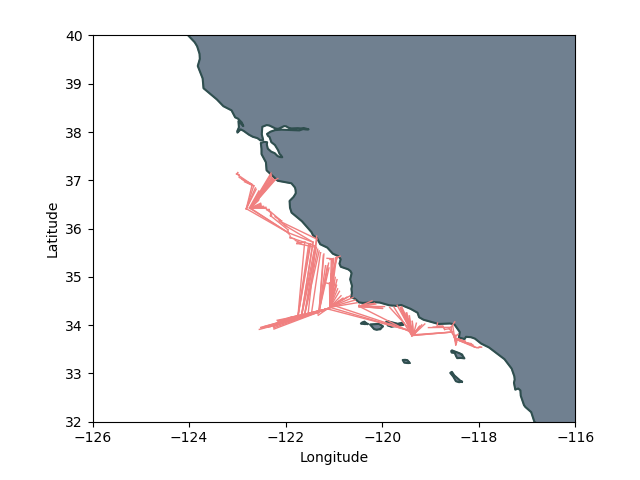
\includegraphics[width=.45\columnwidth]{fig/lasf_search_iter500.png}
    }
    \subfloat[6000 iterations]{
      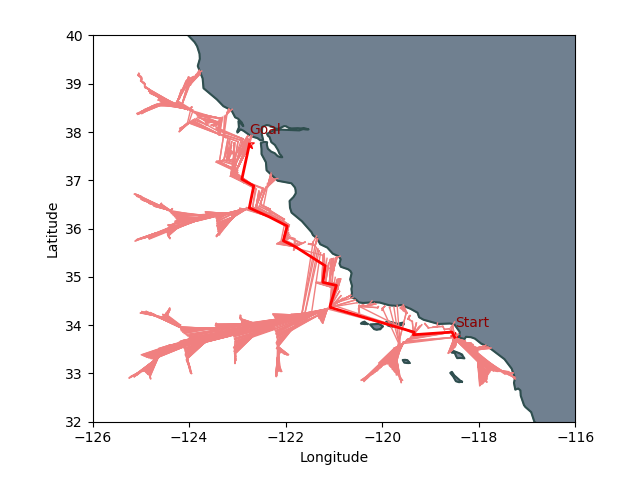
\includegraphics[width=.45\columnwidth]{fig/lasf_search_iter6000.png}
    }
    \caption{LA to SF planning search graph.}
    \label{fig:lasf_search}
\end{figure}

\begin{figure}[!ht]
    \centering
    \subfloat[500 iterations]{
      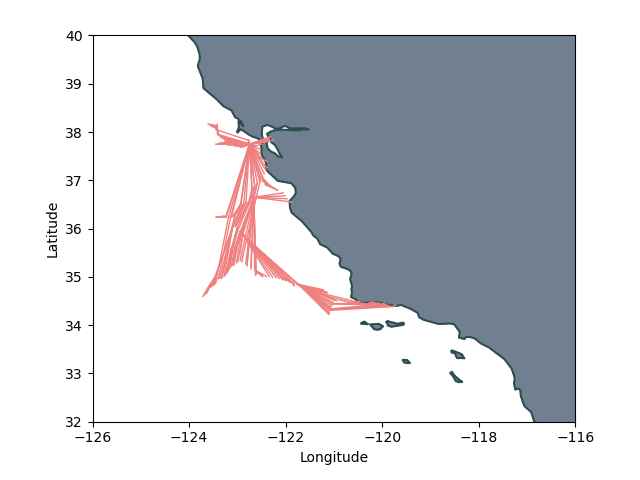
\includegraphics[width=.45\columnwidth]{fig/sfla_search_iter500.png}
    }
    \subfloat[6000 iterations]{
      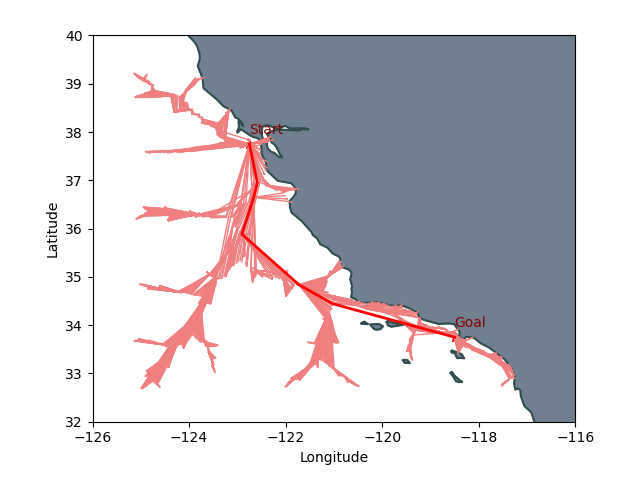
\includegraphics[width=.45\columnwidth]{fig/sfla_search_iter6000.png}
    }
    \caption{SF to LA planning search graph.}
    \label{fig:sfla_search}
\end{figure}

A route off of the coast of California between Los Angeles (LA) and San Francisco (SF) was used as a medium-distance test case. Figures \ref{fig:lasf_search} and \ref{fig:sfla_search} depict the search graphs generated by the RRT* algorithm for these cases, and Figure \ref{fig:routes} depicts the resulting optimal routes. The weather at the starting time is also plotted, but keep in mind that the weather is time-varying in reality.

\begin{figure}[!ht]
    \centering
    \subfloat[LA to SF]{
      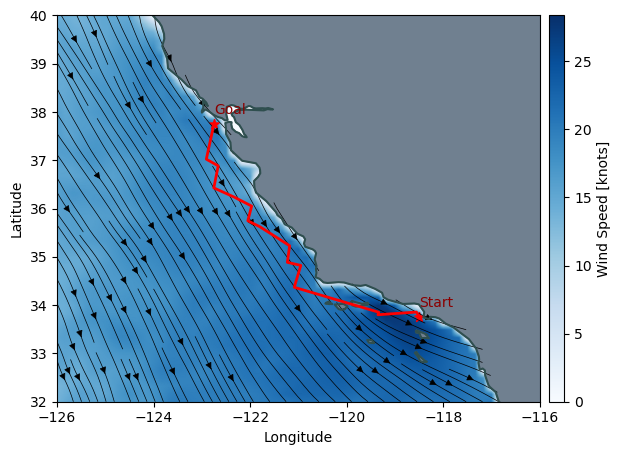
\includegraphics[width=65mm]{fig/lasf_route.png}
    }
    \hspace{0mm}
    \subfloat[SF to LA]{
      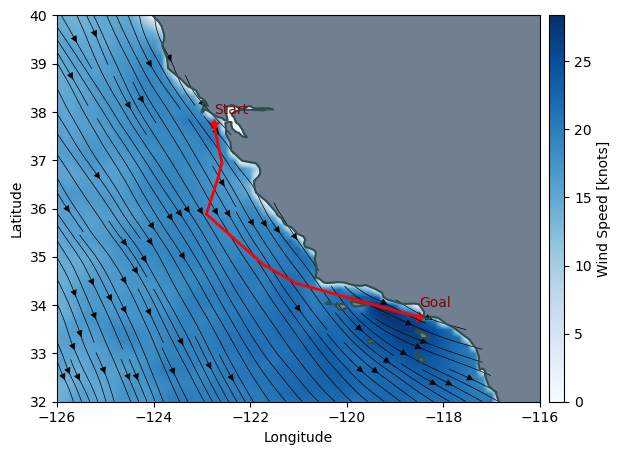
\includegraphics[width=65mm]{fig/sfla_route.png}
    }
    \caption{Optimized routes.}
    \label{fig:routes}
\end{figure}

From LA to SF, the boat was going mainly upwind, and we can see that the optimized route generated tacking behavior. This route achieved a route duration of 2 days and 16 hours at an average speed of 6.37 knots. In the other direction, from SF to LA, the boat was going mainly downwind and generated a much more direct route. This route achieved a duration of 2 days and 10 hours at an average speed of 6.40 knots.

\section{Trajectory Optimization}
\label{section:trajectory_optimization}
To generate an optimal trajectory locally along the path of waypoints from our route planning, we implemented 3 methods of trajectory optimization: direct collocation (DIRCOL), time-optimized DIRCOL, and Iterative Linear Quadratic Regulator (iLQR).
\subsection{Direct Collocation}
DIRCOL trajectory optimization is a method that discretizes the system dynamics and control inputs over a finite number of time steps. The process involves formulating dynamic constraints and an objective function, discretizing the dynamics equations, parameterizing the control inputs, and then solving the resulting optimization problem to find the trajectory that minimizes the objective while satisfying the constraints. This approach allows for handling the nonlinear dynamics of a sailboat and complex constraints efficiently. Our objective function:

\begin{equation}
\resizebox{\linewidth}{!}{$
\begin{aligned}
\min_{x_{1:N},u_{1:N-1}} \quad & \sum_{i=1}^{N-1} \bigg[ \frac{1}{2} (x_i - x_{\text{goal}})^TQ(x_i -x_{\text{goal}}) + \frac{1}{2} u_i^TRu_i \bigg] + \frac{1}{2}(x_N - x_{\text{goal}})^TQ_f(x_N -x_{\text{goal}}) \\ 
\text{s.t.} \quad & x_1 = x_{\text{IC}}, \\
& f_{hs}(x_i,x_{i+1},u_i,dt) = 0 \quad \text{for } i = 1,2,\ldots,N-1, \\
& \frac{-\pi}{3} \leq u_i \leq \frac{\pi}{3} \quad \text{for } i = 1,2,\ldots,N-1.
\end{aligned}
$}
\end{equation}

minimizes the cost between our current state to goal state to find the most optimal dynamically feasible trajectory.

\begin{figure}[!ht]
    \centering
    \subfloat[Trajectory]{
      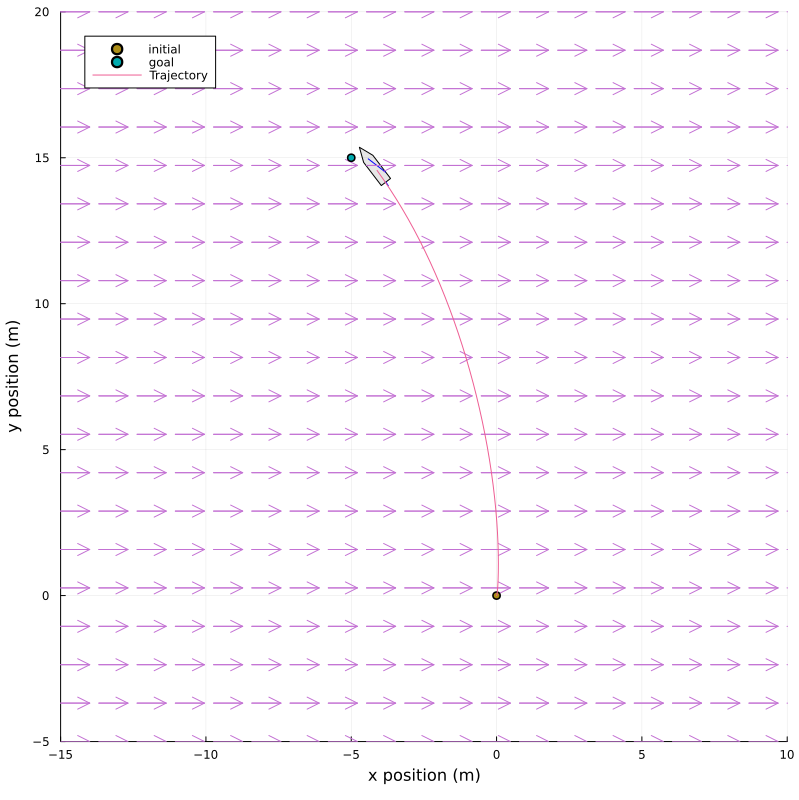
\includegraphics[width=65mm]{fig/dircol_trajectory.png}
    }
    \hspace{0mm}
    \subfloat[Control Input]{
      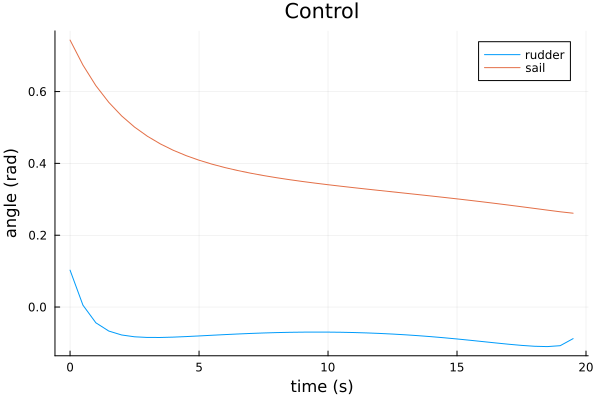
\includegraphics[width=65mm]{fig/dircol_control.png}
    }
    \caption{DIRCOL optimized trajectory.}
    \label{fig:dircol}
\end{figure}

\subsection{Time-optimized Direct Collocation}
Time-optimized direct collocation extends the traditional DIRCOL method by introducing an additional optimization variable: the time allocation along the trajectory. Instead of using a fixed time grid, time-optimized direct collocation allows for the simultaneous optimization of both the trajectory and the time at each time step. This enables the system to adaptively allocate time to different segments of the trajectory, potentially reducing the overall execution time. By optimizing both the control inputs and the time allocation, this approach can lead to more efficient and dynamically feasible trajectories.

\begin{figure}[!ht]
    \centering
    \subfloat[Trajectory]{
      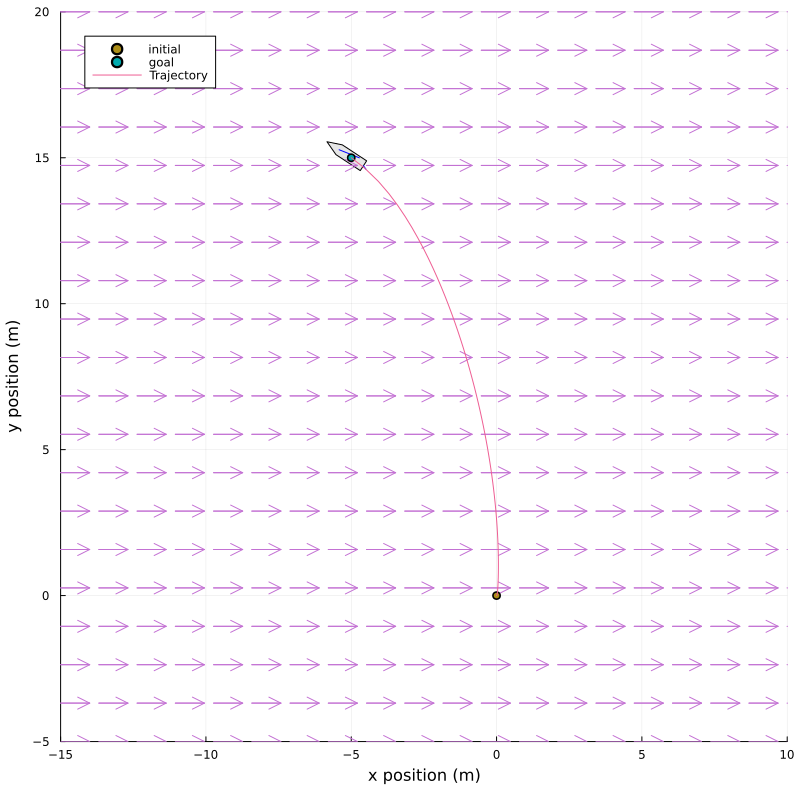
\includegraphics[width=65mm]{fig/timopt_trajectory.png}
    }
    \hspace{0mm}
    \subfloat[Control Input]{
      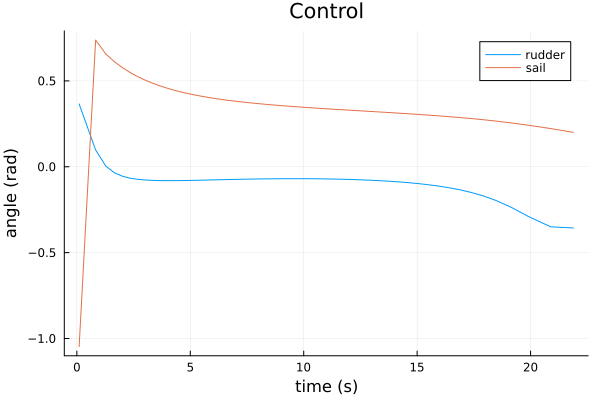
\includegraphics[width=65mm]{fig/timeopt_control.png}
    }
    \caption{Time-optimized DIRCOL trajectory.}
    \label{fig:timeopt-dircol}
\end{figure}

\subsection{Iterative Linear Quadratic Regulator}
Iterative Linear Quadratic Regulator (iLQR) trajectory optimization is a powerful method used to find optimal control sequences for nonlinear dynamical systems. It operates iteratively, refining the control inputs to improve the performance of the system iteratively. At each iteration, iLQR linearizes the dynamics of the system around a nominal trajectory and then computes optimal control inputs using the Linear Quadratic Regulator (LQR) framework, which is designed for linear systems. These locally optimal control inputs are then applied to the system, and the process iterates, with the linearization and optimization steps repeated until convergence. iLQR can handle complex constraints and is robust to nonlinearity, making it suitable for complex sailboat dynamics. Its iterative nature allows for refining the trajectory incrementally, leading to improved performance and efficiency over successive iterations.

\subsection{Results}
Overall, from testing various trajectory optimization methods from a given set of way-points Fig \ref{fig:timeopt-dircol} shows that the Time-optimized DIRCOL trajectory optimization method performed the best. Within a given number of time-steps the method was able to optimize the time between each step and the control inputs to ensure the sailboat achieved its goal in an optimal trajectory. This proved to be a problem for the vanilla DIRCOL method as it would require an accurate discretization of time and steps to achieve the goal or the boat would overshoot or stray away from the goal as seen in Fig \ref{fig:dircol}. Finally iLQR struggled with the same time aspect as vanilla DIRCOL and relied heavily on the quality of the initial guess to the control inputs, which would cause the control inputs to be heavily unstable and infeasible throughout the trajectory.

\section{Tracking Control}
\label{section:tracking_control}
The purpose of the tracking controller is to compute the control inputs that steer the sailboat in a way that minimizes the deviation from the reference trajectory which is obtained from the DIRCOL optimization. The tracking controller is implemented using model predictive control (MPC). MPC is chosen due to its ability to handle constraints and work over a finite horizon which allows it to run in real time.

The MPC controller is implemented in python using the CVXPY library. This controller takes the A and B matrices that come from linearizing the system dynamics and finds the optimal input that minimizes a quadratic cost function, while adhering to the constraints such as input limits and dynamics.

\begin{equation}
\resizebox{\linewidth}{!}{$
\begin{aligned}
\min_{x_{1:N}, u_{1:N-1}} \quad & \sum_{i=1}^{N-1} \left[ \frac{1}{2} (x_i - x_{\text{goal}})^T Q (x_i - x_{\text{goal}}) + \frac{1}{2} u_i^T R u_i \right] + \frac{1}{2} (x_N - x_{\text{goal}})^T Q_f (x_N - x_{\text{goal}}) \\ 
\text{s.t.} \quad & x_{k+1} = A_k x_k + B_k u_k, \\
& -\frac{\pi}{3} \leq u_i \leq \frac{\pi}{3} \quad \text{for } i = 1, 2, \ldots, N-1.
\end{aligned}
$}
\end{equation}

\begin{itemize}
    \item \( Q = 0.03 \cdot I_{nx} \) where \( I_{nx} \) is the \( nx \times nx \) identity matrix,
    \item \( R = 0.05 \cdot I_{nu} \) where \( I_{nu} \) is the \( nu \times nu \) identity matrix,
    \item \( Q_f = 10 \cdot I_{nx} \) where \( I_{nx} \) is the \( nx \times nx \) identity matrix again.
\end{itemize}

\section{Conclusion}
This project presents a comprehensive approach to the optimal control of autonomous sailboats, aiming to contribute to the realization of carbon-neutral shipping solutions. Leveraging real-world weather predictions and innovative control strategies, our system demonstrates the potential for sailboats to become a competitive and sustainable autonomous option in the shipping industry. By employing optimal techniques throughout the stack---RRT* for planning, direct collocation for trajectory optimization, and model predictive control for tracking---we created a robust and tightly integrated control system.

\subsection{Future Work}

One of the advantages of the optimal control framework which our system is built on is that we can easily add many types of constraints and cost functions. Future work could expand on this front, adding collision avoidance with other ships, or avoiding hurricane areas for instance. Additionally, within this framework, we can potentially make safety and performance guarantees.

We would also like to expand our dynamics to be more representative of real-world vessels and conditions. For example, we are not currently modeling Eddy damping, an assumption that holds for small to medium vessels \cite{ModelingCourseControl}. However, as we are interested in the modeling and control of large shipping vessels, this is likely not a safe or conservative assumption. This is one of many such areas that can be further developed and refined.

\section*{Acknowledgment}
Thank you to Zachary Manchester for the insightful lectures and project advising.

\FloatBarrier
\printbibliography

\newpage
\appendix

\subsection{Dynamics parameters}

\begin{table}[ht]
\centering
\begin{tabular}{c|c|c}
\textbf{Parameter} & \textbf{Description} & \textbf{Value} \\
\hline & \\[-6pt]
    $\rho_w$    & water density & 1025 $\frac{kg}{m^3}$ \\[4pt]
    $\rho_a$    & air density   & 1.23 $\frac{kg}{m^3}$ \\[4pt]
    $g$         & gravity       & 9.81 $\frac{m}{s^2}$  \\[4pt]
\hline & \\[-6pt]
    $m$             & mass          & 1.6e3 $kg$        \\[4pt]
    $I_{xx}$        & inertia       & 6.8e3 $kg\ m^2$   \\[4pt]
    $I_{zz}$        & inertia       & 8.5e3 $kg\ m^2$   \\[4pt]
    $X_{\dot{u}}$   & added mass    & -1.6e2 $kg$       \\[4pt]
    $Y_{\dot{v}}$   & added mass    & -1.2e3 $kg$       \\[4pt]
    $K_{\dot{p}}$   & added mass    & -1.0e3 $kg\ m^2$  \\[4pt]
    $N_{\dot{r}}$   & added mass    & -2.4e3 $kg\ m^2$  \\[4pt]
    $Y_{\dot{p}}$   & added mass    & 0 $kg\ m$         \\[4pt]
    $Y_{\dot{r}}$   & added mass    & -3.5e2 $kg\ m$    \\[4pt]
\hline & \\[-6pt]
    $A_s$       & sail area             & 23.8 $m^2$    \\[4pt]
    $A_k$       & keel area             & 0.93 $m^2$    \\[4pt]
    $A_r$       & rudder area           & 0.30 $m^2$    \\[4pt]
    $l_1$       & CoM to sail base      & -1.82 $m$     \\[4pt]
    $l_2$       & sail base to sail CoE & 1.35 $m$      \\[4pt]
    $l_3$       & CoM to keel CoE       & -0.66 $m$     \\[4pt]
    $l_4$       & CoM to rudder CoE     & 3.7 $m$       \\[4pt]
    $h_1$       & height to sail CoE    & 5.2 $m$       \\[4pt]
    $h_2$       & height to keel CoE    & 0.95 $m$      \\[4pt]
    $h_3$       & height to rudder CoE  & 0.7 $m$       \\[4pt]
\hline & \\[-6pt]
    $\nabla$    & water displacement            & 1.568 $m^3$                   \\[4pt]
    $GM_t$      & transverse metacentric height & 2.4 $m$                       \\[4pt]
    $d_{11}$    & linear damping constant       & 10.0 $\frac{kg\ m}{s}$        \\[4pt]
    $d_{22}$    & linear damping constant       & 16.0 $\frac{kg\ m}{s}$        \\[4pt]
    $d_{66}$    & linear damping constant       & 40.0 $\frac{kg\ m^2}{rad\ s}$ \\[4pt]
\hline & \\[-6pt]
    $Re_c$              & current Renolds number    & 1e6  $-$              \\[4pt]
    $S_H$               & wetted surface area       & 9.8 $m^2$             \\[4pt]
    $k$                 & hull form factor          & 0.15 $-$              \\[4pt]
    $C_D$               & Damping drag coefficient  & 1.0 $m$               \\[4pt]
    $C_L$               & Damping lift coefficient  & 1.0 $m$               \\[4pt]
    $L$                 & hull length               & 8.8 $m$               \\[4pt]
    $T$                 & constant draft            & 1.0 $m$               \\[4pt]
    $B_{FO}$            & $v=0$ damping coefficient & 15.0 $-$              \\[4pt]
    $B_L$               & Lift damping in roll      & 70.0 $\frac{kg}{rad}$ \\[4pt]
    $L_{WL}$            & Length of waterline       & 8.8 $m$               \\[4pt]
    $\omega_{roll_n}$   & natural frequency in roll & 2.4 $\frac{1}{s}$     \\[4pt]
\hline
\end{tabular}
\label{tab:dynamics_parameters}
\end{table}

\end{document}